\documentclass{article}
\usepackage{amsmath}
\usepackage{amssymb}
\usepackage{geometry}
\usepackage{xcolor}
\usepackage{mdframed}
\geometry{a4paper, margin=1in, bottom=1cm}
\usepackage{multirow}
\usepackage{array}
\usepackage{booktabs}
\usepackage{tikz}
\usepackage{adjustbox}

\title{Problemas de Asignación}
\author{Ricardo Largaespada}
\date{19 de noviembre 2024}

\newmdenv[
  backgroundcolor=blue!5,
  linecolor=blue,
  linewidth=1pt,
  roundcorner=5pt,
  skipabove=\baselineskip,
  skipbelow=\baselineskip
]{problem}

\begin{document}

\maketitle

\vspace{-1cm}
\begin{problem}
El entrenador de un equipo de natación debe asignar competidores para la prueba de 200 metros de relevo combinado que irá a las Olimpiadas Juveniles. Como muchos de sus mejores nadadores son rápidos en más de un estilo, no es fácil decidir cuál de ellos asignar a cada uno de los cuatro estilos. Los cinco mejores nadadores y sus mejores tiempos (en segundos) en cada estilo son los siguientes:

\begin{center}
\begin{tabular}{|c|c|c|c|c|c|}
\hline
\textbf{Tipo de nado} & \textbf{Carl} & \textbf{Chris} & \textbf{David} & \textbf{Tony} & \textbf{Ken} \\
\hline
Dorso & 37.7 & 32.9 & 33.8 & 37.0 & 35.4 \\
\hline
Pecho & 43.4 & 33.1 & 42.2 & 34.7 & 41.8 \\
\hline
Mariposa & 33.3 & 28.5 & 38.9 & 30.4 & 33.6 \\
\hline
Libre & 29.2 & 26.4 & 29.6 & 28.5 & 31.1 \\
\hline
\end{tabular}
\end{center}

El entrenador quiere determinar cómo asignar cuatro nadadores a los cuatro estilos de nado para minimizar la suma de los mejores tiempos correspondientes.

\begin{enumerate}
    \item[a)] Formule este problema como uno de asignación.
    \item[b)] Obtenga una solución óptima.
\end{enumerate}

\end{problem}

\vspace{-1cm}

\begin{problem}
    La figura muestra la distribución esquemática de un taller con sus centros de trabajo existentes designados por los cuadrados 1, 2, 3 y 4. Se tienen que agregar cuatro nuevos centros de trabajo, \( I \), \( II \), \( III \) y \( IV \), al taller en los lugares designados por los círculos \( a \), \( b \), \( c \) y \( d \).

\begin{center}
    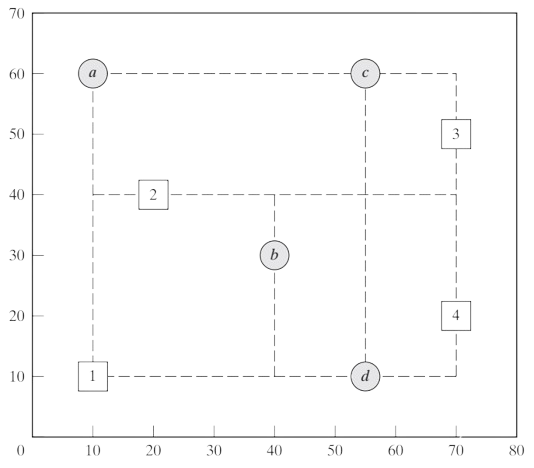
\includegraphics[width=8cm]{distribution.png} % Usa una imagen para la figura 5.5
\end{center}

El objetivo es asignar los nuevos centros a los lugares propuestos para minimizar el tráfico total de manejo de materiales entre los centros existentes y los propuestos. La tabla 5.41 resume la frecuencia de los viajes entre los centros nuevos y los anteriores:

\begin{center}
\begin{tabular}{|c|c|c|c|c|}
\hline
\textbf{Centro existente} & \textbf{I} & \textbf{II} & \textbf{III} & \textbf{IV} \\
\hline
1 & 10 & 2 & 4 & 3 \\
\hline
2 & 7 & 1 & 9 & 5 \\
\hline
3 & 0 & 8 & 6 & 2 \\
\hline
4 & 11 & 4 & 0 & 7 \\
\hline
\end{tabular}
\end{center}

El equipo de manejo de materiales viaja a lo largo de los pasillos rectangulares que se cortan en las ubicaciones de los centros. Por ejemplo, la distancia del viaje en un sentido (en metros) entre el centro 1 y la ubicación \( b \) es \( 30 + 20 = 50 \, \mathrm{m} \).
\end{problem}

\end{document}
